\chapter{Related Work}

\section{Text-to-Image Generation}

Most of the recent research on text-to-image generators has focused on generating photorealistic images \citep{zhang2017stackgan,ramesh2021zeroshot,johnson2018image,zhao2019image,mansimov2015generating,oord2016conditional,oord2016pixel,reed2016learning} using machine learning approaches such as Generative Adversarial Networks -- GANs \citep{zhang2017stackgan,zhao2019image}, Cascaded Refinement Networks -- CRNs \citep{johnson2018image} or autoregressive models \citep{ramesh2021zeroshot,oord2016conditional,oord2016pixel}.
However, these models are limited to generating low-resolution images, e.g., $32\times32$ \citep{mansimov2015generating,oord2016conditional,oord2016pixel}, $64\times64$ \cite{johnson2018image,oord2016pixel}, $128\times128$ \citep{reed2016learning}, $256\times256$ \citep{zhang2017stackgan,ramesh2021zeroshot}. Some approaches do not generate images directly from the text but use intermediate structures such as scene graphs \citep{johnson2018image,tripathi2019using} or layouts \citep{zhao2019image}. 

\begin{figure}[ht]
    \centering
    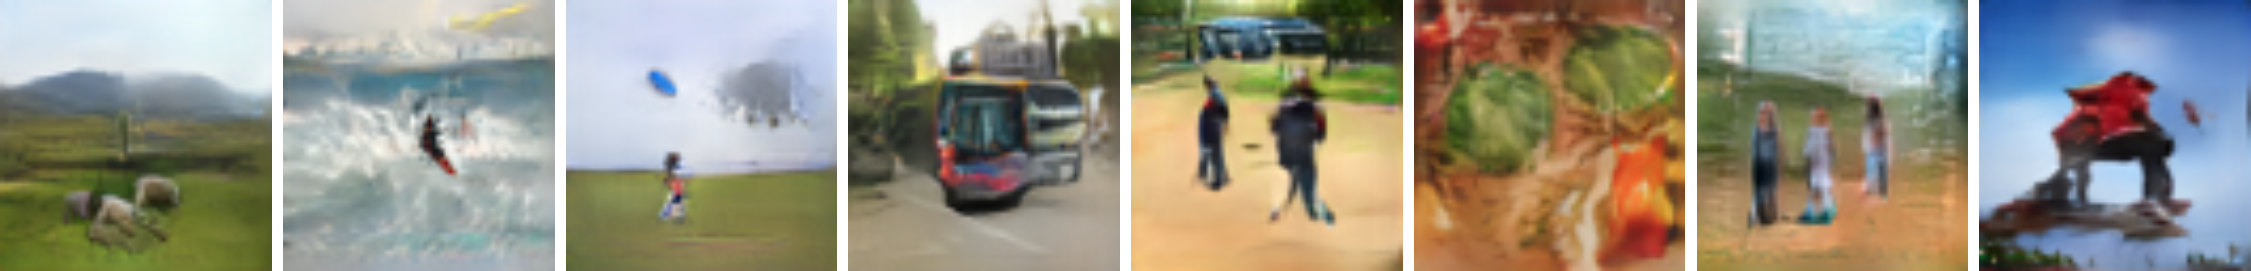
\includegraphics[width=\textwidth]{figures/johnson.png}
    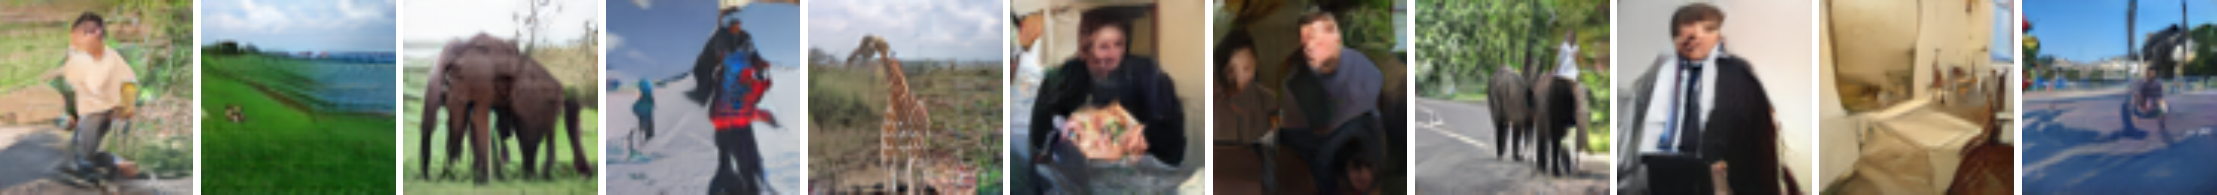
\includegraphics[width=\textwidth]{figures/zhao.png}
    \caption[Generated photorealistic images]{Examples of generated photorealistic images. Top row: Johnson et al. \cite{johnson2018image}, bottom row: Zhao et al. \cite{zhao2019image}.}
    \label{fig:photorealistic_examples}
\end{figure}


\section{Scene Graphs}

A scene graph is a graph-based representation of a scene, where vertices of the graph are objects and edges are relations between objects. Scene graphs have been used for image retrieval \citep{schuster2015generating,johnson2015image}, image generation \citep{johnson2018image}, improving \citep{Liu_2017} or evaluating \citep{anderson2016spice} image captions. Schuster et al.  \citep{schuster2015generating}, proposed rule-based and \break classifier-based approaches for converting sentences to scene graphs with no significant performance difference between the two. We use our own yet similar rule-based approach for text-to-scene graph conversion.

\begin{figure}[ht]
    \centering
    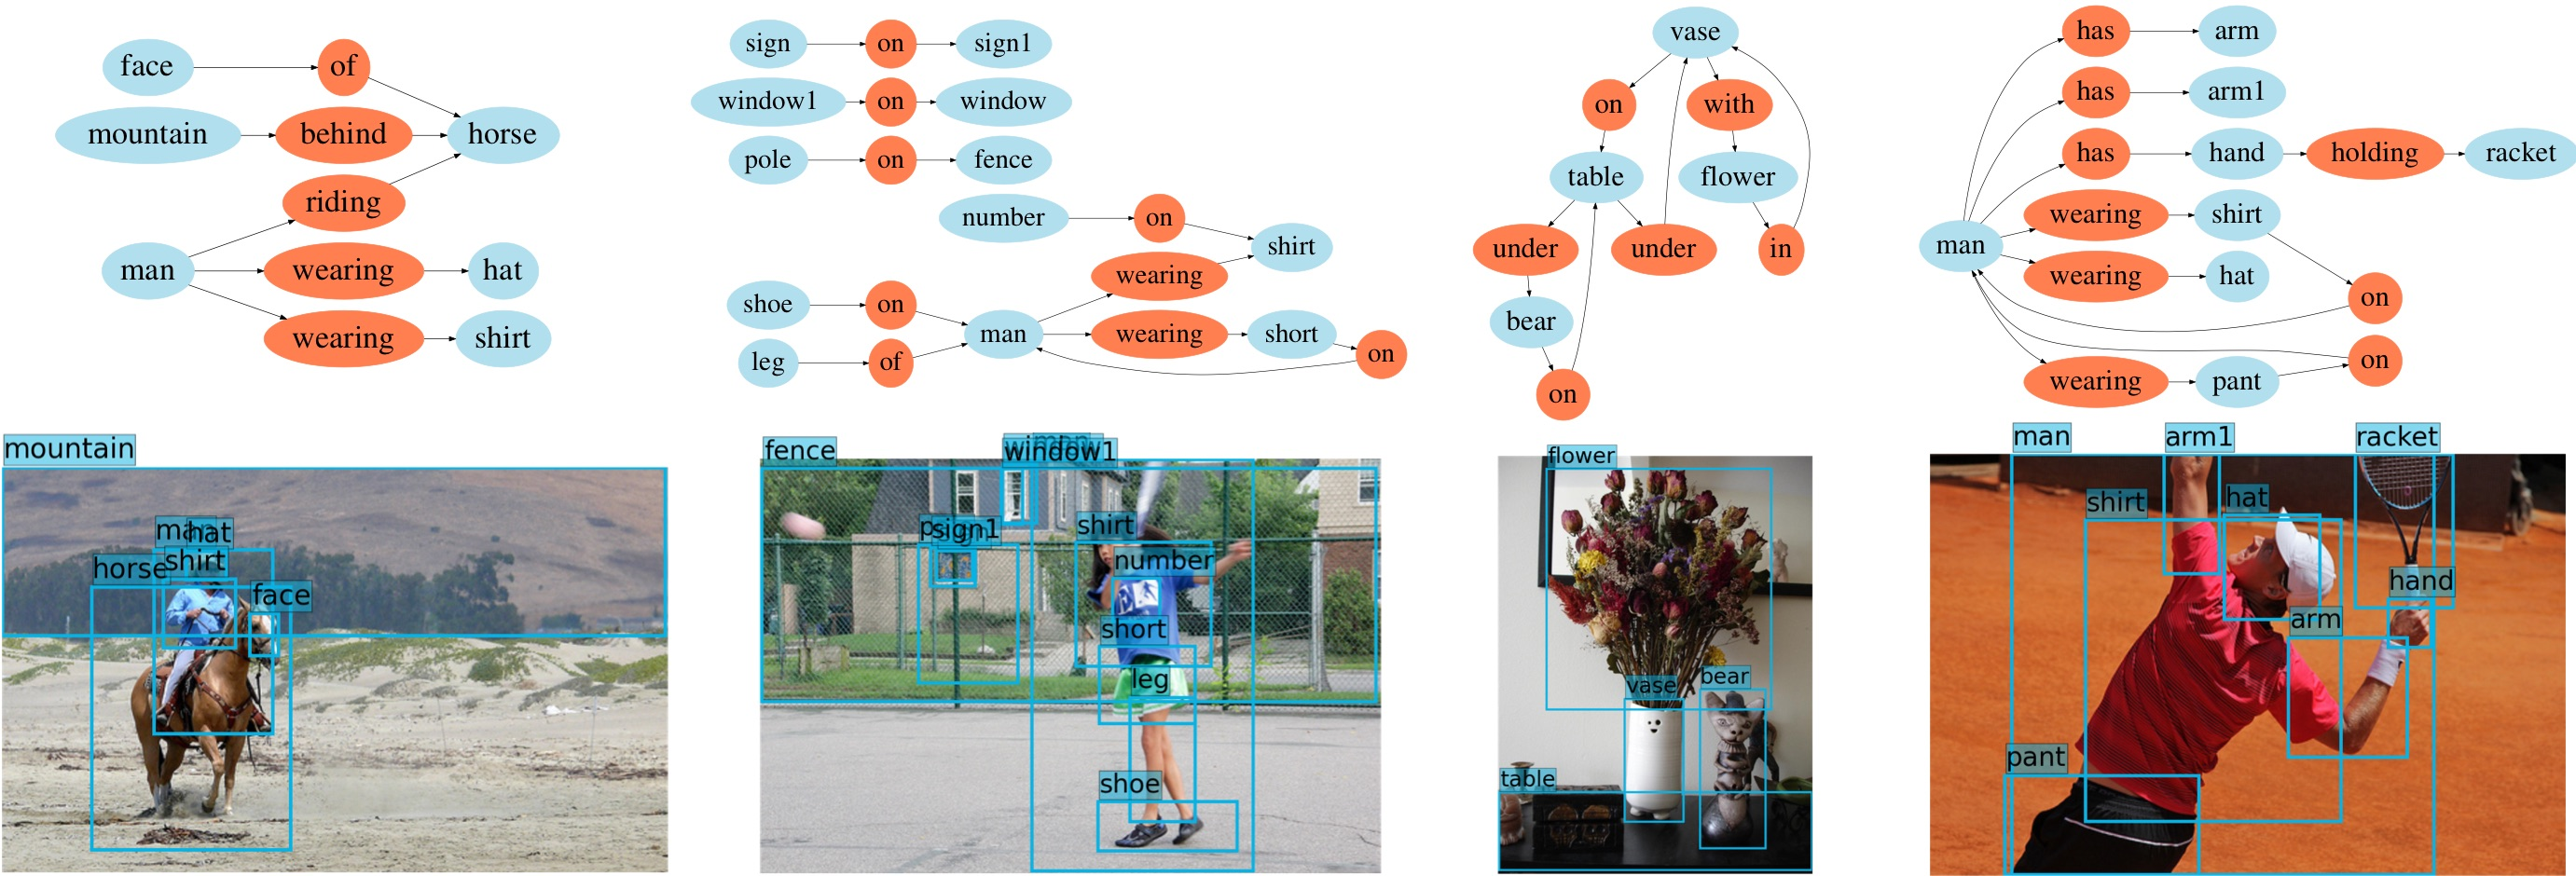
\includegraphics[width=\textwidth]{figures/scene_graph.jpeg}
    \caption[Examples of scene graphs]{Examples of scene graphs from the \emph{Scene Graph} dataset.\footref{footnote:quickdraw} \citep{xu2017scenegraph}}
    \label{fig:scene_graph_example}
\end{figure}
\addtocounter{footnote}{1}
\footnotetext{Image taken from the \emph{Scene Graph} dataset webpage \url{https://cs.stanford.edu/~danfei/scene-graph/}.\label{footnote:quickdraw}}

\medskip

Most work on scene graphs is based on \emph{Visual Genome}  \citep{krishnavisualgenome} dataset, which contains scene graphs annotated by humans. This thesis uses \emph{Scene Graph}  \citep{xu2017scenegraph} dataset based on the \emph{Visual Genome}. Unlike the original dataset, this dataset is deprived of ambiguous object names and poor quality bounding boxes.

\section{Drawing Datasets}

Google's \emph{Quick, Draw!} \citep{quickdraw} dataset is the largest hand-drawn sketch dataset at the time. It contains 50 million individual drawings classified into 345 categories. The \emph{Quick, Draw!} dataset provides the broadest range of categories compared to other widely used datasets such as \emph{TU-Berlin} \citep{eitz2012hdhso} dataset with 250 categories and \emph{Sketchy} \citep{sketchy2016} dataset with 125 categories.

\medskip

The \emph{Quick, Draw!} \citep{quickdraw} dataset contains sketches of common objects represented as sets of pen strokes. \Cref{fig:quickdraw_example} shows a sample of sketches present in the dataset.

\begin{figure}[ht]
    \centering
    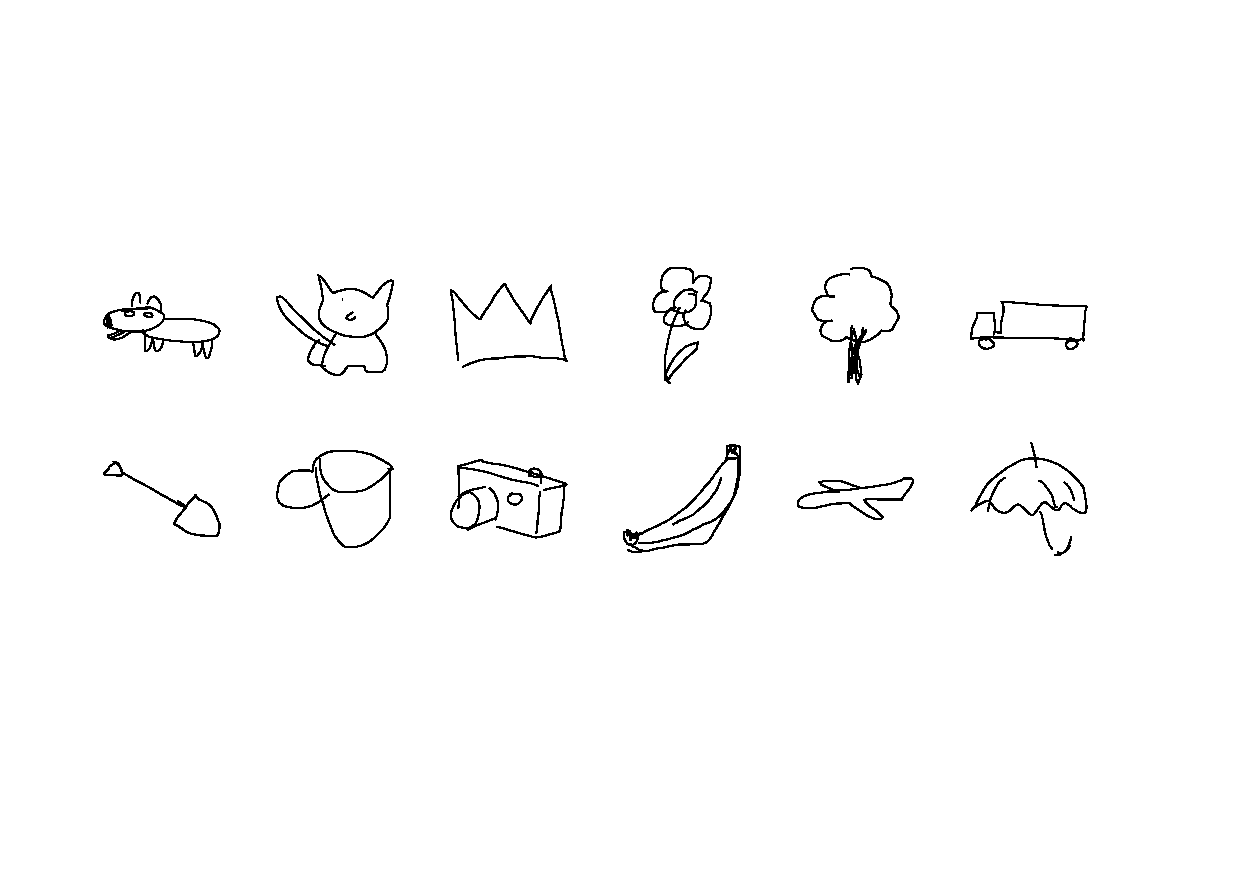
\includegraphics[width=\textwidth,trim=40 150 40 125,clip]{figures/quickdraw.pdf}
    \caption[Sample of drawings from the \emph{Quick, Draw!} dataset]{Sample of drawings from the \emph{Quick, Draw!} dataset.}
    \label{fig:quickdraw_example}
\end{figure}
